\documentclass[a4paper,11pt]{article}
\usepackage{a4wide}
\usepackage{fullpage}
\usepackage[utf8x]{inputenc}

%\usepackage[light,math]{anttor}
\usepackage[T1]{fontenc}

\usepackage[slovene]{babel}
%\selectlanguage{slovene}
\usepackage[toc,page]{appendix}
\usepackage[pdftex]{graphicx} 

\usepackage{lmodern}
\usepackage{amsmath}
\usepackage{amssymb}
\usepackage{amsthm}
\usepackage{amsfonts}
\usepackage{mathtools}
\usepackage{enumitem}
\usepackage{amsfonts}
\usepackage{amsmath}
\usepackage{setspace}
\usepackage{relsize}
\usepackage{color}
\definecolor{light-gray}{gray}{0.95}
\usepackage{listings} 
\usepackage{hyperref}
\renewcommand{\baselinestretch}{1.2} 
\renewcommand{\appendixpagename}{Priloge}

\lstset{ 
language=Matlab,
basicstyle=\footnotesize,
basicstyle=\ttfamily\footnotesize\setstretch{1},
backgroundcolor=\color{light-gray},
}

%\usepackage{algorithm}
%\usepackage[noend]{algpseudocode}

\theoremstyle{definition} 
\newtheorem*{definicija}{Definicija}
\newtheorem*{trditev}{Trditev}


\theoremstyle{plain} 
\newtheorem*{izrek}{Izrek}
\newtheorem*{posledica}{Posledica}
\newtheorem*{zgled}{Zgled}
\newtheorem{primer}{Primer}

\title{Krožnica in ostale stožnice \\
v racionalni B\'ezierjevi obliki
}
\author{Sara Bizjak in Urša Blažič}
\date{\today}

%%%%%%%%%%%%%%%%%%%%%%%%%%%%%%%%%%%%%%%%%%%%%%%%%%%%%%%%%%%%%%%%%%%%%%%%%%%%%%%%%%%%%%

\begin{document}

\maketitle

\section{Uvod}
V seminarski nalogi so predstavljene krožnice in ostale stožnice v racionalni B\'ezierjevi obliki. Med tem ko so stožnice na splošno omenjene le v grobem, pa se v krožnice bolj poglobimo in jih podamo natančneje.

Najprej se na splošno seznanimo z racionalnimi B\'ezierjevimi krivuljami in jih poslošimo na stožnice. Iz stožnic preidemo na krožnico in si jo natančeneje pogledamo. Ugotovimo, kako lahko dobimo sklenjeno krožnico z racionalno krivuljo čim nižje stopnje in jo konstruiramo.


%%%%%%%%%%%%%%%%%%%%%%%%%%%%%%%%%%%%%%%%%%%%%%%%%%%%%%%%%%%%%%%%%%%%%%%%%%%%%%%%%%%%%%

\section{Racionalne B\'ezierjeve krivulje}

Racionalna B\'ezierjeva krivulja stopnje $n$ v $\mathbb{R}^d$ je projekcija polinomske B\'ezierjeve krivulje stopnje $n$ v $\mathbb{R}^{d+1}$ na hiperravnino $w=1$, kjer točko v  $\mathbb{R}^{d+1}$  označimo z
$$(\boldsymbol{x},w)=(x_1,x_2,\dots,x_d,w).$$
Projekcija je definirana kot
$$(\boldsymbol{x},w)\mapsto (\frac{1}{w}\boldsymbol{x},1).$$
Točke oblike $\lambda(\boldsymbol{x}, w)$ za $\lambda\neq 0$ se preslikajo v isto točko na projektivni ravnini, točke z
$w = 0$ pa predstavljajo točke v neskončnosti.

\begin{definicija}
\emph{Racionalna B\'ezierjeva krivulja} stopnje $n$ je podana s parametrizacijo $\boldsymbol{r}:[0,1]\rightarrow \mathbb{R}^d$, določeno s predpisom
$$\boldsymbol{r}(t)=\frac{\mathlarger{\sum}_{i=0}^n w_i\boldsymbol{b}_iB_i^n(t)}{\mathlarger{\sum}_{i=0}^n w_iB_i^n(t)},$$
kjer so $\boldsymbol{b}_i$ kontrolne točke krivulje, $w_i\in\mathbb{R}^d$ uteži, $B_i^n$ pa $i$-ti Bernsteinov bazni polinom stopnje~$n$.
\end{definicija}
 
Krivuljo lahko brez škode za splošnost reparametriziramo tako, da sta $w_0$ in $w_n$ enaka $1$. Taki obliki pravimo \emph{standardna oblika} racionalne B\'ezierjeve krivulje.
Ostale uteži so prosti parametri, ki vplivajo na obliko krivulje -- s povečanjem enega izmed $w_i$ se krivulja približa ustreznemu $\boldsymbol{b}_i$. Racionalne B\'ezierjeve krivulje s pozitivnimi utežmi imajo podobne lastnosti kot polinomske. 

%%%%%%%%%%%%%%%%%%%%%%%%%%%%%%%%%%%%%%%%%%%%%%%%%%%%%%%%%%%%%%%%%%%%%%%%%%%%%%%%%%%%%%

\section{Stožnice v racionalni B\'ezierjevi obliki}
Stožnice bomo zapisali s pomočjo krivulje stopnje $2$, zato bo kontrolni poligon sestavljen iz treh kontrolni točk. Ker lahko izberemo uteži v standardni obliki, velja: 
$$w_0=w_2=1 $$
in
$$ w_1=w,$$
kjer je $w_1$ prosta utež.
\\
Stožnice lahko zapišemo v racionalni B\'ezierjevi obliki kot 
$$\boldsymbol{r}(t)=\frac{\boldsymbol{b}_0\cdot B_0^2+w\cdot\boldsymbol{b}_1\cdot B_1^2+\boldsymbol{b}_2\cdot B_2^2}{ B_0^2+w\cdot B_1^2+ B_2^2}\,\, t\in[0,1],$$
kjer so $\boldsymbol{b}_0, \boldsymbol{b}_1, \boldsymbol{b}_2 \in \mathbb{R}^2$ kontrolne točke krivulje, $w$ utež, vezana na kontrolno točko $\boldsymbol{b}_1$, $B_i^2,\,i=~0,1,2,$ pa Bernsteinovi bazni polinomi:

\begin{align*}
B_0^2(t) &= (1-t)^2 \\
B_1^2(t) &= 2t\cdot(1-t) \\
B_2^2(t) &= t^2 \\
\end{align*}

Ker uteži, kot že omenjeno, izbiramo v standardni obliki, je srednja utež $w_1$ prosti parameter, ki vpliva na obliko krivulje. Če utež $w_1$ povečujemo, se krivulja približuje kontrolni točki $b_1$ kot je prikazano na sliki \ref{slika:w1}.

\begin{figure}[ht!]\label{slika:w1}
    \centering
    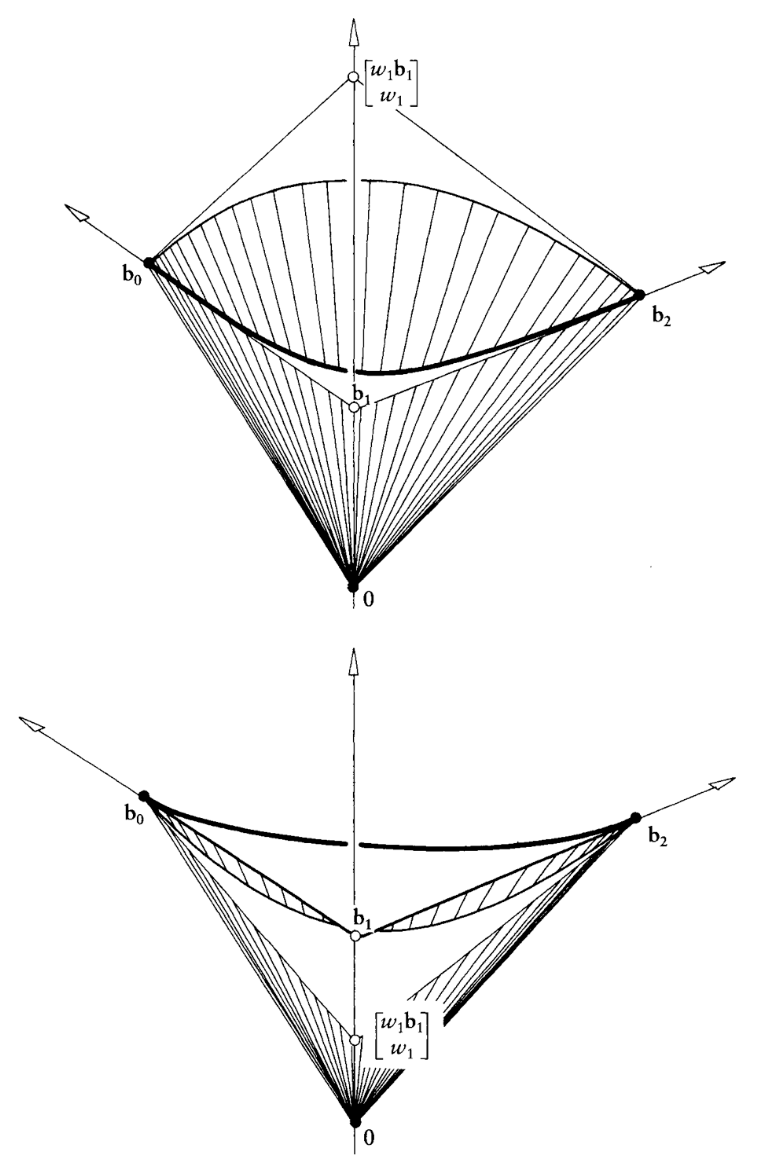
\includegraphics[width=70mm]{vecanje_w1.png}
    \caption{Krivulji na obeh slikah sta v standardni obliki, torej velja $w_0 = w_2 = 1$. Sliki prikazujeta večanje uteži $w_1$, to je približevanje krivulje k kontrolni točki $b_1$. Slika je povzeta po \cite{farin}.}
\end{figure}

\newpage
Spreminjanjae uteži $w_1$ in vpliv na obliko krivuljo lahko klasificiramo v tri skupine. Če je $w_1 < 1$, ima krivulja obliko elipse, če je $w_1 = 1$ je krivulja parabola, za $w_1 > 1$ pa dobimo hiperbolo. Omenjeni trije tipi krivulj so prikazani na sliki \ref{slika:klasifikacija}.

\begin{figure}[ht!]\label{slika:klasifikacija}
    \centering
    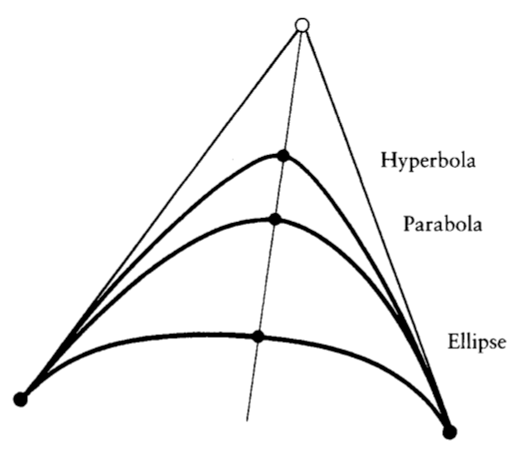
\includegraphics[width=70mm]{tri_oblike.png}
    \caption{Klasifikacije krivulje glede na spreminjanje srednje uteži $w_1$ pri predpostavki, da velja $w_0 = w_2 = 1$. Slika je povzeta po \cite{farin}.}
\end{figure}
\noindent
Ena izmed najpomembnejših stožnic je krog, zato mu v nadaljevanju posvetimo več pozornosti.


%%%%%%%%%%%%%%%%%%%%%%%%%%%%%%%%%%%%%%%%%%%%%%%%%%%%%%%%%%%%%%%%%%%%%%%%%%%%%%%%%%%%%%

\section{Krožnica v racionalni B\'ezierjevi obliki}

\subsection{Motivacija}

Naj kvadratična krivulja z utežjo $w_1 < 1$ opiše krožni lok. Ker je krog simetričen, mora kontrolni poligon tvoriti enakostranični trikotnik.
Če poznamo kot v trikotniku, označimo ga z $\alpha$, lahko določimo utež $w_1$ kot $w_1 = \text{cos} \alpha$.
Celoten krog lahko tedaj predstavimo kot zlepek večih takih krožnih lokov. 

\begin{figure}[ht!]\label{slika:krogpodelih}
    \centering
    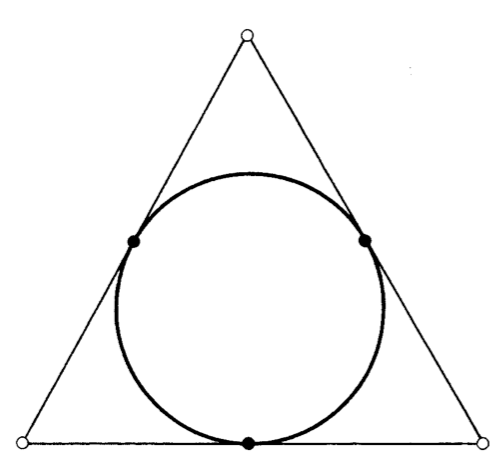
\includegraphics[width=60mm]{krog_po_delih.png}
    \caption{Celoten krog lahko sestavimo iz treh racionalnih kvadratičnih B\'ezierjevih krivulj. Slika je povzeta po \cite{farin}.}
\end{figure}
\noindent
Na sliki \ref{slika:krogpodelih} je prikazan primer, ko je kot $\alpha$ velik 60 stopinj, torej velja $w_1 = \frac{1}{2}$. V tem primeru je krog sestavljen iz treh enakih krožnih lokov.
\\

Namesto, da krožnico opisujemo z zlepkom krivulj, bi jo želeli opisati z eno samo racionalno krivuljo čim nižje stopnje.
\\
Nadalje si najprej oglejmo formalno definicijo krožnice v racionalni B\'ezierjevi obliki in problem iskanja racionalne krivulje čim nižje stopnje, ki opiše krožnico, reducirajmo na lažjega.

\subsection{Formulacija krožnice v racionalni B\'ezierjevi obliki}
Krožnico lahko opišemo kot racionalno B\'ezierjevo krivuljo $C(t)=(X(t),Y(t))$ s pomočjo projekcije krivulje $\tilde{C}(t)=(\tilde{X}(t), \tilde{Y(t)}, W(t))$ na ravnino $w=1$. 
Enačbo krožnice v $\mathbb{R}^2$ lahko zapišemo kot
$$X(t)^2+Y(t)^2=1$$
Koordinate točk zamenjamo s koordinatami prostora $\mathbb{R}^3$, ki smo jih dobili s projekcijo na ravnino $w=1$.
$$\left(\frac{\tilde{X}(t)}{W(t)}\right)^2+\left(\frac{\tilde{Y}(t)}{W(t)}\right)^2=1$$
$$\tilde{X}(t)^2+\tilde{Y}(t)^2-W(t)^2=0$$
Zadnja enačba predstavlja enačbo stožca. Vidimo, da racionalna krivulja $C(t)$ eksaktno opiše krožnico kot projekcijo krivulje $\tilde{C}(t)$ (ki leži na stožcu) na ravnino $w = 1$.
\\
\\
SLIKA stožca
\\
\\
Iskanje racionalne krivulje čim nižje stopnje, ki eksaktno opiše celotno krožnico, lahko torej prevedemo na problem iskanja krivulje, ki leži na stožcu. 

%%%%%%%%%%%%%%%%%%%%%%%%%%%%%%%%%%%%%%%%%%

\subsection{ Kvadratična krivulja}
Pokazali bomo, da racionalna kvadratična krivulja ne more opisati celotne krožnice. Vse neracionalne kvadratične B\'ezierjeve krivulje so parabole, vse parabole pa dobimo kot presek stožca z ravnino, ki je vzporedna eni od nosilk stožca. Ko ravnino, s katero presekamo stožec, premikamo proti nosilki stožca, opazimo, da bo krožni lok v projekciji  na ravnino opisal vedno večji kot, torej smo vedno bližje polnemu krogu. Ko pa naredimo presek ravnine z nosilko stožca, je presek premica, ki se v projekciji slika v eno točko. Krožnice zato ne moremo zapisati s kvadratično racionalno krivuljo. 

Opazimo, da lahko s parabolo zapišemo krožne loke, ki jih lahko opišemo z naslednjim kontrolnim poligonom:
\begin{align*}
\boldsymbol{\tilde{P}}_0 &= (cos(\theta), -sin(\theta), 1)\\
\boldsymbol{\tilde{P}}_1 &= (1, 0, cos(\theta))\\
\boldsymbol{\tilde{P}}_2 &= (cos(\theta), sin(\theta), 1),
\end{align*}
kjer je $\theta$ polovični kot krožnega loka. Če izberemo samo pozitivne uteži ($\cos{\theta}>0$), je $C(t)$ manj kot $180^{\circ}$, če pa je srednja utež enaka $0$ ($\cos{\theta}=0$), je $C(t)$ točno $180^{\circ}$. ??
% Za prvo in zadnjo točko si izberemo točki, ki ležita na krožnici, srednjo točko pa zaradi simetrije izberemo na polovičnem kotu med njima. Pri tem izberemo take uteži, da zadoščajo enačbi stožca. 

%%%%%%%%%%%%%%%%%%%%%%%%%%%%%%%%%%%%%%%%%%

\subsection{Kubična krivulja}
Pokazali bomo, da tudi racionalna kubična krivulja ne more opisati celotne krožnice. \\
Za kontrolni poligon potrebujemo štiri kontrolne točke. S krivuljo interpoliramo prvo in zadnjo kontrolno točko, izberemo ju na stožcu.
????

%%%%%%%%%%%%%%%%%%%%%%%%%%%%%%%%%%%%%%%%%%

\subsection{Krivulja 4.~stopnje}
Da bomo dobili vse krivulje, v enačbo za stožec $\tilde{X}(t)^2+\tilde{Y}(t)^2-W(t)^2=0$ vstavimo ??? \\
Bernsteinove bazne polinome $B_i^8(t),\,i=0,\ldots,8$ enačimo z $0$ in dobimo devet enačb.
Brez škode za splošnost vzamemo $\boldsymbol{\tilde{P}}_0 =\boldsymbol{\tilde{P}}_4 = (1,0,1)$. Ker $\boldsymbol{\tilde{P}}_1$ in $\boldsymbol{\tilde{P}}_3$ ležita v tangentni ravnini $\boldsymbol{\tilde{P}}_0$, velja $\tilde{x}_1=w_1$ in $\tilde{x}_3=w_3$ (saj imamo ravnino $x=w$). Devet enačb se nam tako reducira v pet enačb:
\begin{align*}
\tilde{y}_3 &=- \tilde{y}_1 \\
\tilde{x}_3 &= - \tilde{x}_1 \\
3\tilde{x}_2 + 4\tilde{y}_1^2 - 3w_2 &= 0 \\
\tilde{x}_1\tilde{x}_2 + \tilde{y}_1\tilde{y}_2  - \tilde{x}_1w_2 &= 0 \\
9\tilde{x}_2^2 - 8\tilde{y}_1^2 + 9\tilde{y}_2^2 - 9w_2^2&= 0 \\
\end{align*}
Iz zadnjih treh enačb dobimo dve možni rešitvi
\begin{align*}
\tilde{y}_1 &= \alpha \\
\tilde{x}_2 &=-\frac{3w_2-4\tilde{x}_1^2+2}{3}\\
\tilde{y}_2 &= \frac{4}{3}\tilde{x}_1\alpha
\end{align*}
in
\begin{align*}
\tilde{y}_1 &= -\alpha \\
\tilde{x}_2 &=-\frac{3w_2-4\tilde{x}_1^2+2}{3}\\
\tilde{y}_2 &= -\frac{4}{3}\tilde{x}_1\alpha
\end{align*}

kjer je $\alpha=(\frac{3w_2}{2}-\tilde{x}_1^2+\frac{1}{2})^{\frac{1}{2}}$

Dobimo naslednje kontrolne točke, ki tvorijo kontrolni poligon:
\begin{align*}
\boldsymbol{\tilde{P}}_0 &= (1,0,1) \\
\boldsymbol{\tilde{P}}_1 &= (\tilde{x}_1,\pm\alpha,\tilde{x}_1) \\
\boldsymbol{\tilde{P}}_2 &= (-\frac{3w_2-4\tilde{x}_1^2+2}{3},\pm\frac{4}{3}\tilde{x}_1\alpha,w_2) \\
\boldsymbol{\tilde{P}}_3 &= (-\tilde{x}_1,\mp\alpha,-\tilde{x}_1) \\
\boldsymbol{\tilde{P}}_4 &= (1,0,1)
\end{align*}

Ker mora biti $\alpha$ pozitivno število, mora veljati
$$w_2>-\frac{1}{3}$$
in
$$-\left(\frac{3w_2+1}{2}\right)^{\frac{1}{2}}<\tilde{x}_1<\left(\frac{3w_2+1}{2}\right)^{\frac{1}{2}}$$
Vidimo, da zaradi $\boldsymbol{\tilde{P}}_1$ in $\boldsymbol{\tilde{P}}_3$ nikoli ne dobimo kvartične B\'ezierjeve krivulje z vsemi pozitivnimi utežmi. \\
Če izberemo $\tilde{x}_1=0$, dobimo  
\begin{align*}
\boldsymbol{\tilde{P}}_0 &= (1,0,1) \\
\boldsymbol{\tilde{P}}_1 &= (0,\pm (\frac{1}{2}+\frac{3}{2}w_2)^{1/2},0) \\
\boldsymbol{\tilde{P}}_2 &= (-\frac{2}{3}-w_2,0,w_2) \\
\boldsymbol{\tilde{P}}_3 &= (0,\mp(\frac{1}{2}+\frac{3}{2}w_2)^{1/2},0) \\
\boldsymbol{\tilde{P}}_4 &= (1,0,1)
\end{align*}
V tem primeru nimamo več negativnih uteži, dobimo pa dve uteži, ki sta enaki $0$. Povedali smo že, da točka z $w=0$ pri projekciji na ravnino $w=1$ predstavlja točko v neskončnosti. Torej, imamo dve točki v neskončnosti, tega pa pri implementaciji ne želimo. \\
Kako bi se znebili negativnih uteži? Tako, da dani krivulji dvignemo stopnjo. \\%takrat se bo naš kontrolni poligon pomaknil bližje h krivulji.
Pogoji, da ima taka krivulja same pozitivne uteži, so
$$-\frac{1}{4}<\tilde{x}_1<\frac{1}{4}$$
in
$$-\frac{3}{2}w_2<\tilde{x}_1<\frac{3}{2}w_2.$$

TUKI BI BLO FAJN DAT ŠE KAK PRIMER - SO V ČLANKU

%%%%%%%%%%%%%%%%%%%%%%%%%%%%%%%%%%%%%%%%%%%%%%%%%%%%%%%%%%%%%%%%%%%%%%%%%%%%%%%%%%%%%%

\section{Kubični B\'ezierjev krožni lok}


%%%%%%%%%%%%%%%%%%%%%%%%%%%%%%%%%%%%%%%%%%%%%%%%%%%%%%%%%%%%%%%%%%%%%%%%%%%%%%%%%%%%%%

\begin{thebibliography}{99}
\bibitem{chou}
J.~J.~Chou, \emph{Higher order Bezier circles}, Computer-Aided Design \textbf{27 (4)} (1995) 303--309

\bibitem{farin}
G.~Farin, \emph{Curves and surfaces for CAGD}, A Practical Guide, 5th ed., Morgan Kaufmann, 2002, poglavje 12.7

\bibitem{knez}
M.~Knez, J.~Grošelj, \emph{Računalniško podprto geometrijsko oblikovanje}, ... (2020)
\end{thebibliography}


\end{document}